\documentclass[12pt]{article}
\usepackage[english]{babel}
\usepackage{natbib}
\usepackage{url}
\usepackage[utf8]{inputenc}
\usepackage{amsmath}
\usepackage{amssymb}
\usepackage{graphicx}
\usepackage{parskip}
\usepackage{fancyhdr}
\usepackage{vmargin}
\usepackage{booktabs}
\usepackage[table,xcdraw]{xcolor}
\usepackage{tabularx}
\usepackage{caption} 
\usepackage{float}
\usepackage{longtable}
\usepackage{array}
\usepackage{caption}
\usepackage{subcaption}

\setmarginsrb{3 cm}{1 cm}{3 cm}{1 cm}{1 cm}{1.5 cm}{1 cm}{1.5 cm}

\newcolumntype{L}[1]{>{\raggedright\let\newline\\\arraybackslash\hspace{0pt}}m{#1}}
\newcolumntype{C}[1]{>{\centering\let\newline\\\arraybackslash\hspace{0pt}}m{#1}}
\newcolumntype{R}[1]{>{\raggedleft\let\newline\\\arraybackslash\hspace{0pt}}m{#1}}

\usepackage{natbib}

\title{Assignment \#2 - Distribution Fitting}
\date{\today}

\makeatletter
\let\thetitle\@title
\let\thesubtitle\@subtitle
\let\theauthor\@author
\let\thedate\@date
\makeatother

\pagestyle{plain}

\captionsetup[table]{skip=5pt}


\begin{document}

%%%%%%%%%%%%%%%%%%%%%%%%%%%%%%%%%%%%%%%%%%%%%%%%%%%%%%%%%%%%%%%%%%%%%%%%%%%%%%%%%%%%%%%%%

\begin{titlepage}
	\centering
    \textsc{\LARGE University of Coimbra}\\[1.0 cm]
	\textsc{\large Doctoral Program in Information Science and Technology}\\[0.5 cm]
    \textsc{\large Statistics}\\[5 cm]
	\rule{\linewidth}{0.2 mm} \\[0.4 cm]
	{ \LARGE \bfseries \thetitle}\\ [0.2 cm]
    \rule{\linewidth}{0.2 mm} \\[3 cm]
    
    \textsc{Joaquim Pedro Bento Gonçalves Pratas Leitão - 2011150072}\\[5 cm]
	
	{\large \thedate}\\[2 cm]
 
	\vfill
	
\end{titlepage}

%%%%%%%%%%%%%%%%%%%%%%%%%%%%%%%%%%%%%%%%%%%%%%%%%%%%%%%%%%%%%%%%%%%%%%%%%%%%%%%%%%%%%%%%%

\section{Introduction}
\label{introduction}

The current document is framed in the scope of the second assignment of the Statistics course, taught for the Doctoral Program in Information Science and Technology at the University of Coimbra, during the academic year of 2016/2017. 

In the current assignment a distribution fitting task was proposed. In this task, a probability distribution was intended to be fitted to a collected, and previously provided, dataset.

The dataset in question corresponds to concentrations of Strontium-90 (in micromicrocuries) recorded in 50 samples of milk prepared for consumption by a given company. Taking into account that no prior knowledge regarding the nature or the distribution of the collected data, the approach followed in the current work can be divided in the following steps:

\begin{enumerate}
	\item Identification of potential probability distributions that justify the collected data. At this point, this was accomplished by means of visual inspection, comparing of the histogram of the data with the probability density plots of candidate distributions.
	
	\item Estimation of the parameters of the probability distributions identified in the previous point, based on information extracted from the collected data: At this point, \emph{Maximum Likelihood Estimations} of the parameters will be performed.
	
	\item For each of the probability functions identified in the first point perform the \emph{Kolmogorov-Smirnov} Test, with the parameters estimations obtained in the previous point. The probability distribution chosen to justify the collected data will be the one with the higher \emph{p-value} in the \emph{Kolmogorov-Smirnov} Test.
\end{enumerate}

In the remainder of this document each of these steps will be addressed in an individual section (sections \ref{candidate_distributions} to \ref{ks_test}). In addition, the document will conclude with a brief analysis of the results achieved in this work (section \ref{result_analysis}).

\section{Candidate Probability Distributions}
\label{candidate_distributions}

The current section covers the first step of the adopted approach, where potential probability distribution functions that justify the observed data were identified and selected.

Such functions were selected by comparing the histogram of the observed data with the corresponding probability density functions. Therefore, this section will consist of a very brief presentation of the observed dataset and its corresponding histogram, followed by its analysis and comparison with candidate probability distribution functions.

\subsection{The Dataset}

As already stated in section \ref{introduction}, the dataset provided for this work consisted of concentrations of Strontium-90 (in micromicrocuries) recorded in 50 samples of milk prepared for consumption by a given company. The dataset is presented in table \ref{dataset_table}:

\begin{longtable}{|l|}
		\hline
		Concentration \\ \hline
		7,974   \\ \hline
		9,592   \\ \hline
		7,792   \\ \hline
		8,366   \\ \hline
		8,816   \\ \hline
		7,015   \\ \hline
		8,605   \\ \hline
		7,681   \\ \hline
		9,042   \\ \hline
		6,368   \\ \hline
		6,477   \\ \hline
		8,637   \\ \hline
		8,617   \\ \hline
		6,796   \\ \hline
		7,73    \\ \hline
		7,412   \\ \hline
		8,128   \\ \hline
		11,055  \\ \hline
		4,881   \\ \hline
		7,298   \\ \hline
		11,314  \\ \hline
		10,861  \\ \hline
		8,342   \\ \hline
		6,939   \\ \hline
		5,842   \\ \hline
		10,188  \\ \hline
		6,698   \\ \hline
		6,183   \\ \hline
		8,623   \\ \hline
		10,479  \\ \hline
		7,425   \\ \hline
		9,031   \\ \hline
		4,039   \\ \hline
		9,207   \\ \hline
		7,143   \\ \hline
		8,559   \\ \hline
		5,501   \\ \hline
		11,725  \\ \hline
		6,191   \\ \hline
		5,904   \\ \hline
		5,931   \\ \hline
		7,151   \\ \hline
		9,638   \\ \hline
		8,832   \\ \hline
		7,76    \\ \hline
		8,011   \\ \hline
		7,637   \\ \hline
		7,488   \\ \hline
		8,514   \\ \hline
		9,309   \\ \hline
		\caption{Measured Strontium-90 concentrations.}
		\label{dataset_table}
\end{longtable}

Figure \ref{dataset_histogram} presents the histogram of the observed data:

\begin{figure}[h]
	\centering
	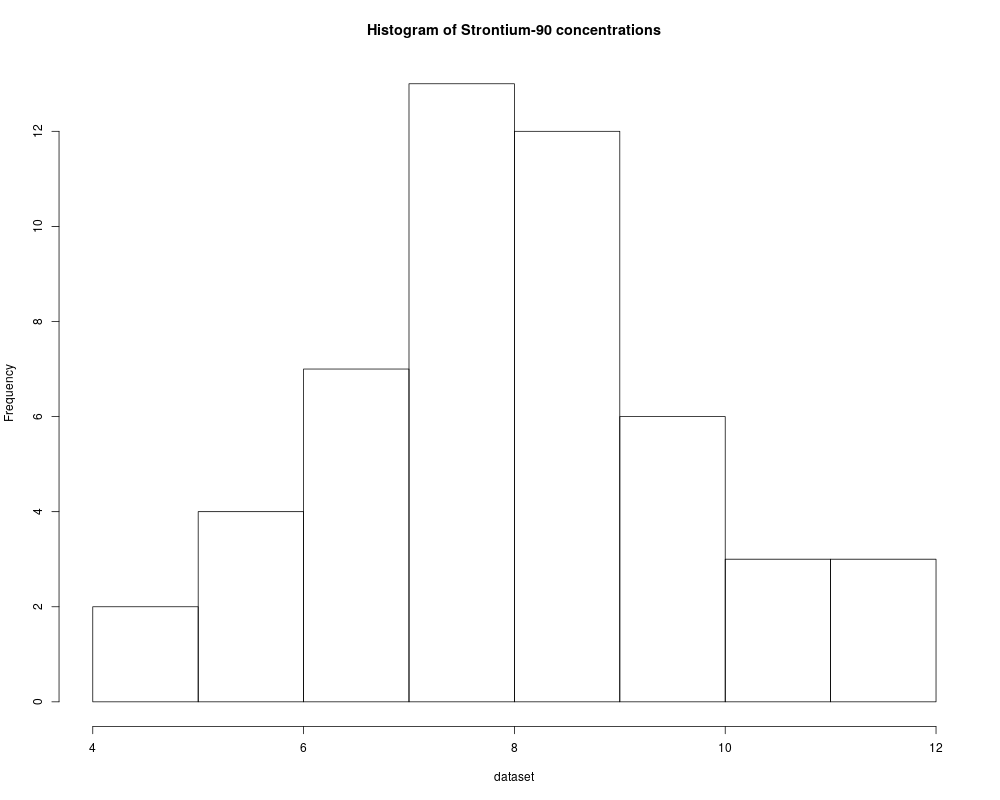
\includegraphics[scale=0.4]{images/Histogram_dataset.png}
	\caption{Histogram of the observed data.}
	\label{dataset_histogram}
\end{figure}

\subsection{Histogram Analysis}

Analysing the histogram presented in figure \ref{dataset_histogram}, a symmetry of the data relative to a value close to 8 is suggested.

Based on this property, symmetric probability distributions were further studied and compared with the obtained histogram. As a result, density functions of several distributions were plotted and compared with this histogram, of which the following distributions were highlighted: \emph{Cauchy}, \emph{Gamma}, \emph{Logistic} and \emph{Normal}.

Figures \ref{histogram_cauchy} to \ref{histogram_normal} presents the histogram of the data overlapped with the density function for each of the mentioned distributions. In order to obtain estimations for the parameters of these distributions the \emph{method of moments} was used.

\begin{figure}[h] 
	\begin{minipage}[b]{0.5\linewidth}
		\centering
		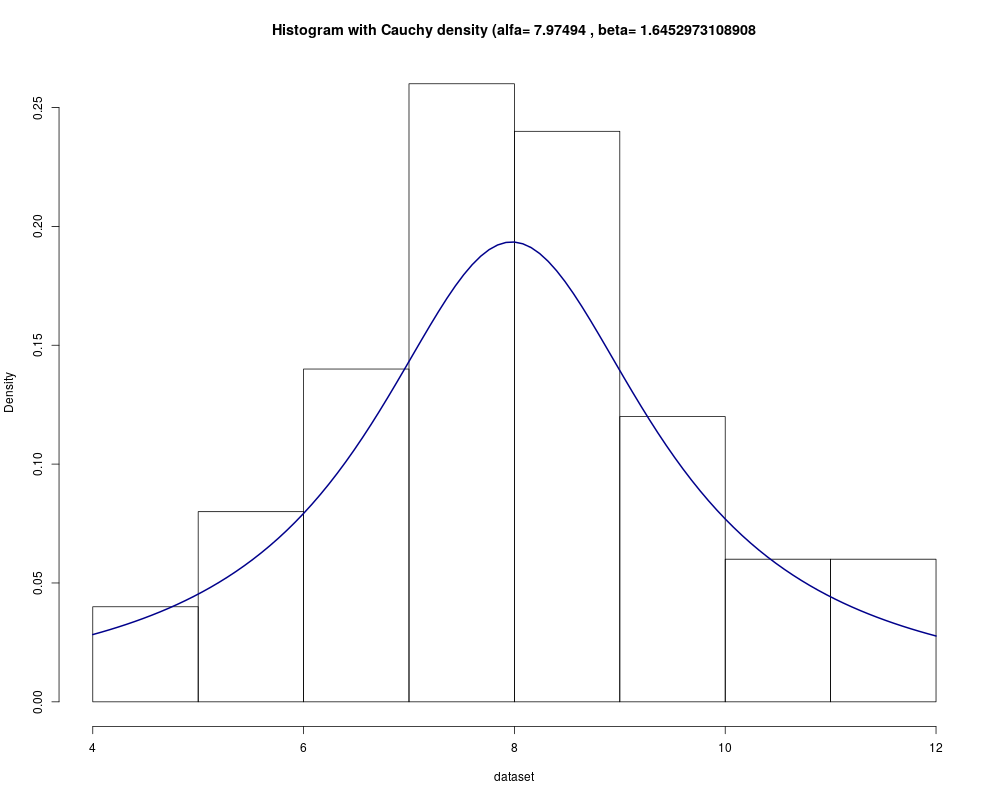
\includegraphics[width=\linewidth]{images/Histogram_Cauchy.png} 
		\caption{Cauchy Distribution.}
		\vspace{4ex}
		\label{histogram_cauchy}
	\end{minipage}%%
	\begin{minipage}[b]{0.5\linewidth}
		\centering
		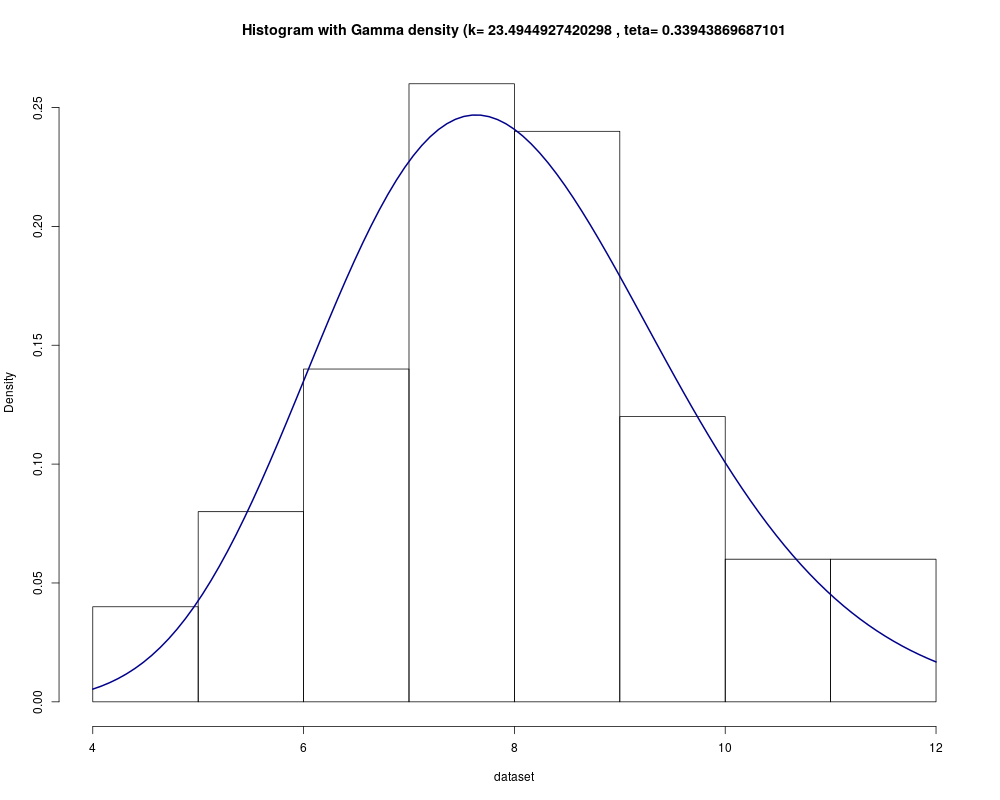
\includegraphics[width=\linewidth]{images/Histogram_Gamma.png} 
		\caption{Gamma Distribution.}
		\vspace{4ex}
		\label{histogram_gamma}
	\end{minipage} 
	\begin{minipage}[b]{0.5\linewidth}
		\centering
		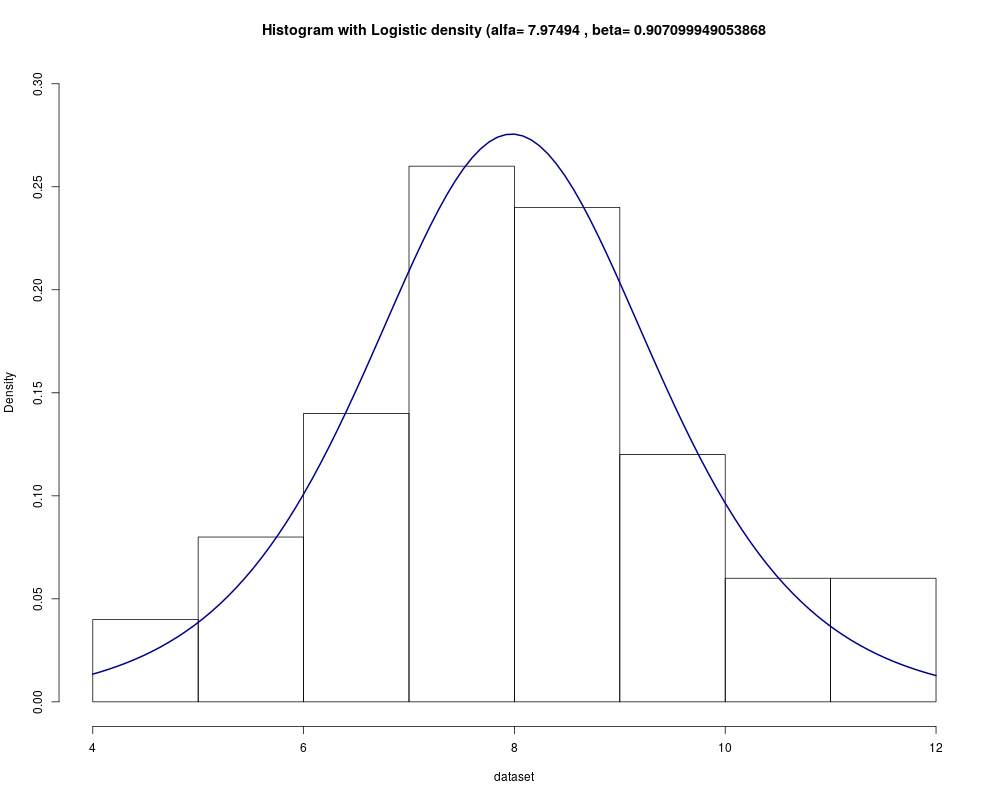
\includegraphics[width=\linewidth]{images/Histogram_Logistic.png} 
		\caption{Logistic Distribution.}
		\vspace{4ex}
		\label{histogram_logistic}
	\end{minipage}%% 
	\begin{minipage}[b]{0.5\linewidth}
		\centering
		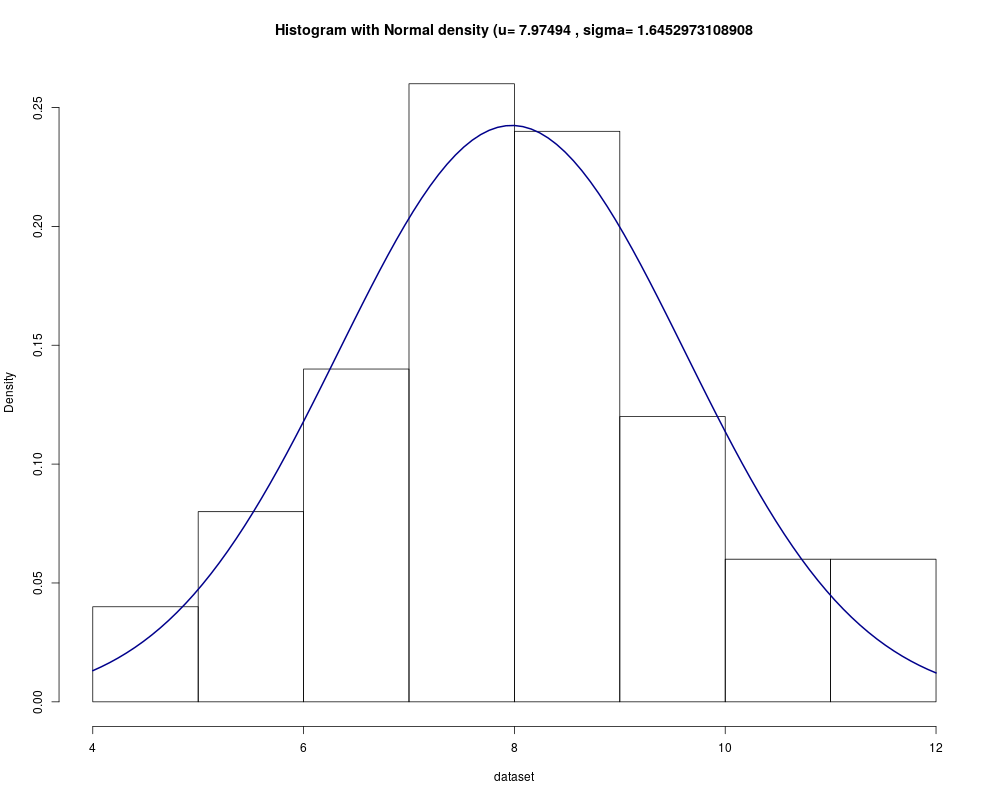
\includegraphics[width=\linewidth]{images/Histogram_Normal.png} 
		\caption{Normal Distribution.}
		\vspace{4ex}
		\label{histogram_normal}
	\end{minipage} 
\end{figure}

From the presented figures it becomes clear that the Cauchy distribution cannot accurately justify the observed data as well as the remaining three distributions. Subsequently, only the Gamma, Logistic and Normal distributions will be considered in the remaining steps of this work.

\section{Parameter Estimation}
\label{parameter_estimations}

Once candidate distributions that seem to justify the observed data were identified, the next logical step to perform is to compute more robust estimations for their parameters, to be used in appropriate statistical tests.

In this work such estimations were obtained by computing \emph{Maximum Likelihood Parameter Estimations} for the three distributions identified in the previous section.

\subsection{Maximum Likelihood Estimations}
\label{maximum_likelihood_estimations}

The \emph{Maximum Likelihood Estimations} were computed using the \emph{R}\footnote{\url{https://www.r-project.org/}} software environment. More precisely, the \emph{mle2} function available in the \emph{bbmle} package was used.

The following estimations were obtained for the considered distributions:

\begin{itemize}
	\item \textbf{Gamma Distribution:} A value of $23.49449$ was estimated for the \emph{shape} parameter \emph{k} and a value of $0.3394412$ was estimated for the \emph{scale} parameter \emph{$\theta$}.
	
	\item \textbf{Logistic Distribution:} A value of $7.946271$ was estimated for the \emph{location} parameter \emph{$\alpha$} and a value of $0.9224431$ was estimated for the \emph{scale} parameter \emph{$\beta$}.
		
	\item \textbf{Normal Distribution:} A value of $7.97494$ was estimated for the \emph{location} parameter \emph{$\mu$} and a value of $1.628762$ was estimated for the \emph{scale} parameter \emph{$\sigma$}.
\end{itemize}

\subsection{QQ-Plots}

A \emph{QQ-Plot} is a graphical method for comparing two probability distributions by plotting their quantiles against each other. If the two distributions being compared are similar, the points in the QQ-Plot will approximately lie on the line $y=x$.

The inclusion of \emph{QQ-Plots} at this stage of the analysis provides additional information regarding the similarity between the observed data and each of the considered distributions.

Figure \ref{qq_plots} presents the obtained \emph{QQ-Plots} for the three distributions, making use of the \emph{maximum likelihood} parameter estimations.

\begin{figure}[h]
	\begin{subfigure}{.5\linewidth}
		\centering
		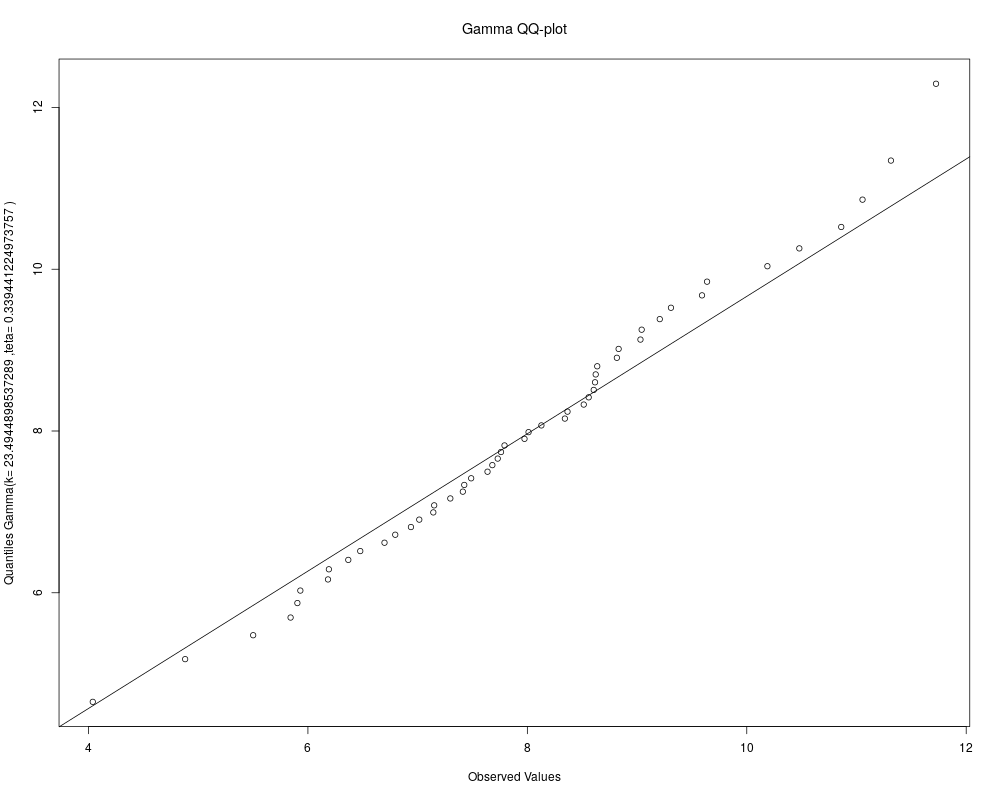
\includegraphics[scale=.2]{images/QQPlot_Gamma.png}
		\label{qq_plot_gamma}
		\caption{Gamma Distribution.}
	\end{subfigure}%
	\begin{subfigure}{.5\linewidth}
		\centering
		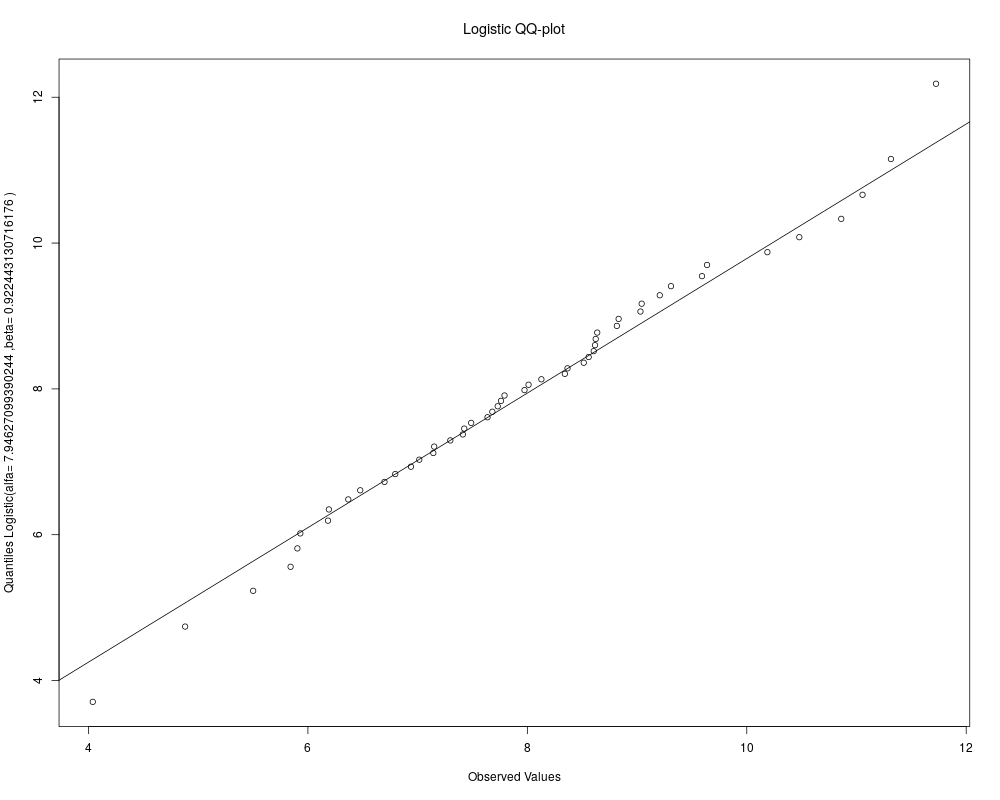
\includegraphics[scale=.2]{images/QQPlot_Logistic.png}
		\label{qq_plot_logistic}
		\caption{Logistic Distribution.}
	\end{subfigure}\\[1ex]
	\begin{subfigure}{\linewidth}
		\centering
		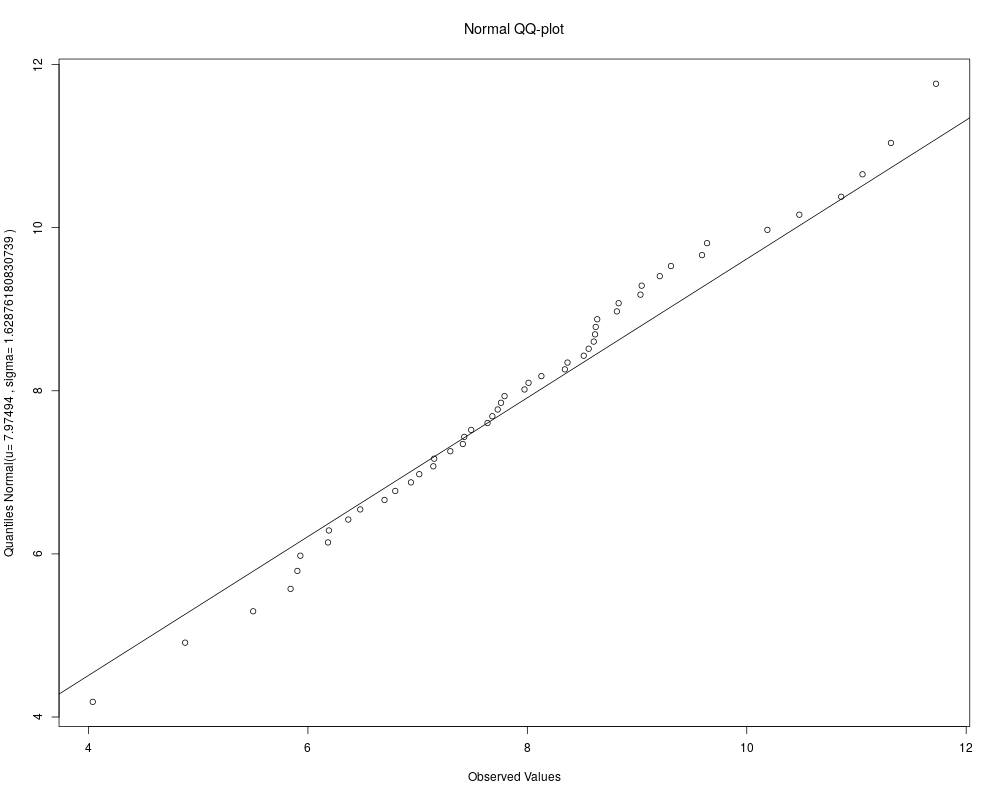
\includegraphics[scale=.2]{images/QQPlot_Normal.png}
		\label{qq_plot_normal}
		\caption{Normal Distribution.}
	\end{subfigure}
	\caption{QQ-Plots with Maximum Likelihood Parameter Estimations.}
	\label{qq_plots}
\end{figure}

Observing the three \emph{QQ-Plots} presented the \emph{Logistic} distribution appears to be the one which better justifies the observed data, as the points in the plot appear to be the ones closer to the line $y=x$.

\section{Kolmogorov-Smirnov Test}
\label{ks_test}

In the final stage of the work, the \emph{Kolmogorov-Smirnov Test} (KS Test) was performed for the three distributions considered. The KS Test is a non-parametric test of equality of continuous, one-dimensional probability distributions, used to compare a sample with a reference probability distribution (one-sample KS Test) or to compare two samples (two-sample KS test).

Considering the data available in the current work, three one-sample KS tests were performed. In these tests the \emph{maximum likelihood parameter estimations} computed in section \ref{maximum_likelihood_estimations} were used. The following \emph{p-value} results were registered:

\begin{itemize}
	\item \textbf{Gamma Distribution:} $p-value=0.9974$
	
	\item \textbf{Logistic Distribution:} $p-value=0.9993$
	
	\item \textbf{Normal Distribution:} $p-value=0.9838$
\end{itemize}

Indeed, in the KS Test, a high \emph{p-value} signals a higher change of the null hypothesis being true, meaning that the higher the \emph{p-value} the more likely the data is to be drawn from the corresponding distribution.

\section{Result Analysis}
\label{result_analysis}

Based on the results of the \emph{Kolmogorov-Smirnov Test} presented in the previous section, and at the significance level of $0.05$, all of the three considered null hypothesis\footnote{Which state that the observed data follows the Gamma, Logistic and Normal distributions.} cannot be rejected. Nevertheless, the test for the Logistic probability distribution registers the higher \emph{p-value}, meaning that this is the most likely distribution that justifies the observed data.

In addition, the Logistic distribution that justifies the observed data, at the significance level of $0.05$ has a \emph{location} parameter $\alpha=7.946271$ and a \emph{scale} parameter $\beta=0.9224431$.

Once a probability distribution has been fitted to the observed data, further questions can be formulated and answered about such data. In the current work the following two questions were raised and, based on the results presented so far in this document, answered:

\begin{enumerate}
	\item \textsl{What is the probability of the concentration of Strontium-90 in milk ranging between 9 and 10 micromicrocuries?}
	
	\item \textsl{What is the concentration of Strontium-90 in milk that has a probability of 0.05 of being exceeded?}
\end{enumerate}

In the first question we want to compute the value of $P(9 \leq X \leq 10)$, where $X$ is a continuous random variable representing the concentration of Strontium-90 in milk (in micromicrocuries). Making use of the cumulative distribution function the previous expression can be written as: $P(9 \leq X \leq 10) = F(10) - F(9)$, yielding a probability of $0.1444894$.

In the second question a value $c \in \mathbb{R}$ is intended to be determined such that $P(X > c) = 0.05$. This expression is equivalent to $P(X \leq c) = 0.95$, which means that we want to find out what is the quantile of order 95 of our continuous random variable $X$. Making use of the \emph{qlogis} function of the \emph{R} software environment, this value can be computed to $10.66235$.

\end{document}